Emacsは伝説の神器です。彼女はエディタであるだけでなく、統合環境でもあります。または開発環境の集大成と呼んでもよいかもしれません。これらの機能はユーザの身を万能のオペレーティングシステムに置きます。

\begin{figure}[H]
  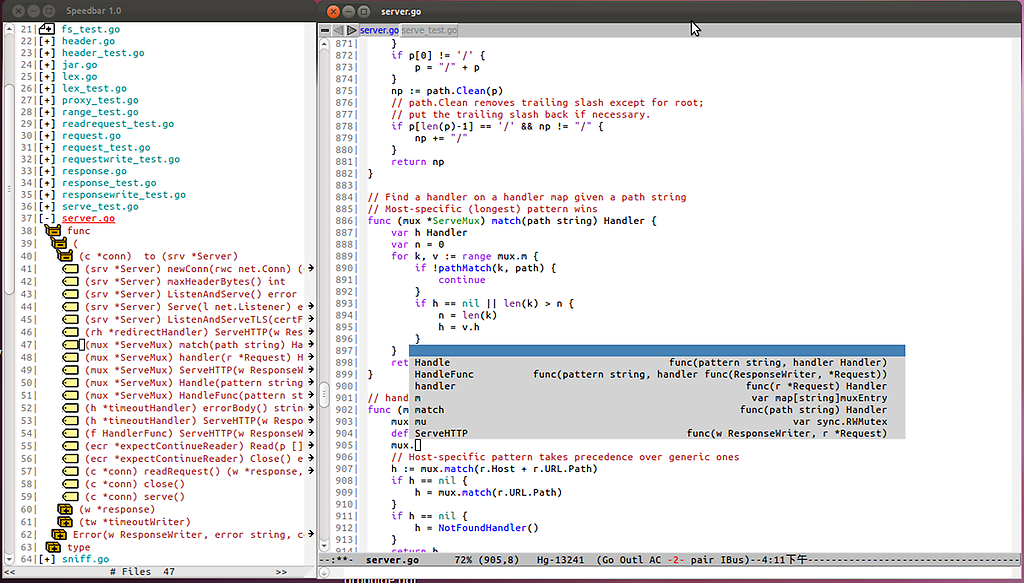
\includegraphics[width=14cm]{1.4.emacs.png}
   \label{図1.10}
   \caption{EmacsでGoを編集するメイン画面}
\end{figure}


\begin{enumerate}
\item Emacsのハイライト表示設定
\begin{lstlisting}[numbers=none]
cp $GOROOT/misc/emacs/* ~/.emacs.d/
\end{lstlisting}
\item Gocodeをインストール
\begin{lstlisting}[numbers=none]
go get -u github.com/nsf/gocode
gocodeはデフォルトで`$GOBIN`の下にインストールされます。
\end{lstlisting}
\item Gocodeを設定
\begin{lstlisting}[numbers=none]
 ~ cd $GOPATH/src/github.com/nsf/gocode/emacs
 ~ cp go-autocomplete.el ~/.emacs.d/
 ~ gocode set propose-builtins true
 propose-builtins true
 ~ gocode set lib-path "/home/border/gocode/pkg/linux_amd64"
                        // あなたのパスに置き換えてください。
 lib-path "/home/border/gocode/pkg/linux_amd64"
 ~ gocode set
 propose-builtins true
 lib-path "/home/border/gocode/pkg/linux_amd64"
\end{lstlisting}
\item Auto Completionをインストールする必要があります。\\ AutoCompleteをダウンロードして解凍します。\\ ~ make install DIR=\$HOME\//.emacs.d\//auto-complete\\ ~\//.emacsファイルを設定します。
\begin{lstlisting}[numbers=none]
;;auto-complete
(require 'auto-complete-config)
(add-to-list 'ac-dictionary-directories
  "~/.emacs.d/auto-complete/ac-dict")
(ac-config-default)
(local-set-key (kbd "M-/") 'semantic-complete-analyze-inline)
(local-set-key "." 'semantic-complete-self-insert)
(local-set-key ">" 'semantic-complete-self-insert)
\end{lstlisting}
詳細情報はこちらを参考にしてください:http://www.emacswiki.org/emacs/AutoComplete
\item .emacsを設定します。
\begin{lstlisting}[numbers=none]
 ;; golang mode
 (require 'go-mode-load)
 (require 'go-autocomplete)
 ;; speedbar
 ;; (speedbar 1)
 (speedbar-add-supported-extension ".go")
 (add-hook
 'go-mode-hook
 '(lambda ()
     ;; gocode
     (auto-complete-mode 1)
     (setq ac-sources '(ac-source-go))
     ;; Imenu & Speedbar
     (setq imenu-generic-expression
         '(("type" "^type *\\([^ \t\n\r\f]*\\)" 1)
         ("func" "^func *\\(.*\\) {" 1)))
     (imenu-add-to-menubar "Index")
     ;; Outline mode
     (make-local-variable 'outline-regexp)
     (setq outline-regexp
       "//\\.\\|//[^\r\n\f][^\r\n\f]\\|pack\\|func\\|impo\\|cons\\|var.\\|type\\|\t\t*....")
     (outline-minor-mode 1)
     (local-set-key "\M-a" 'outline-previous-visible-heading)
     (local-set-key "\M-e" 'outline-next-visible-heading)
     ;; Menu bar
     (require 'easymenu)
     (defconst go-hooked-menu
         '("Go tools"
         ["Go run buffer" go t]
         ["Go reformat buffer" go-fmt-buffer t]
         ["Go check buffer" go-fix-buffer t]))
     (easy-menu-define
         go-added-menu
         (current-local-map)
         "Go tools"
         go-hooked-menu)

     ;; Other
     (setq show-trailing-whitespace t)
     ))
 ;; helper function
 (defun go ()
     "run current buffer"
     (interactive)
     (compile (concat "go run " (buffer-file-name))))

 ;; helper function
 (defun go-fmt-buffer ()
     "run gofmt on current buffer"
     (interactive)
     (if buffer-read-only
     (progn
         (ding)
         (message "Buffer is read only"))
     (let ((p (line-number-at-pos))
     (filename (buffer-file-name))
     (old-max-mini-window-height max-mini-window-height))
         (show-all)
         (if (get-buffer "*Go Reformat Errors*")
     (progn
         (delete-windows-on "*Go Reformat Errors*")
         (kill-buffer "*Go Reformat Errors*")))
         (setq max-mini-window-height 1)
         (if (= 0 (shell-command-on-region
                     (point-min) (point-max)
         "gofmt" "*Go Reformat Output*" nil "*Go Reformat Errors*" t))
     (progn
         (erase-buffer)
         (insert-buffer-substring "*Go Reformat Output*")
         (goto-char (point-min))
         (forward-line (1- p)))
     (with-current-buffer "*Go Reformat Errors*"
     (progn
         (goto-char (point-min))
         (while (re-search-forward "<standard input>" nil t)
         (replace-match filename))
         (goto-char (point-min))
         (compilation-mode))))
         (setq max-mini-window-height old-max-mini-window-height)
         (delete-windows-on "*Go Reformat Output*")
         (kill-buffer "*Go Reformat Output*"))))
 ;; helper function
 (defun go-fix-buffer ()
     "run gofix on current buffer"
     (interactive)
     (show-all)
     (shell-command-on-region (point-min) (point-max)
         "go tool fix -diff"))
\end{lstlisting}
\item おめでとうございます。今からあなたはこの神器を使ってGo開発の楽しみを体験できます。デフォルトのspeedbarは閉じています。もし開く場合は ;; (speedbar 1) の前のコメントを取り去るか、M-x speedbarを手動で起動してください。
\end{enumerate}
